\documentclass[12pt,letterpaper]{article}
\usepackage[margin=1in]{geometry}
\usepackage{caption}
\usepackage[utf8]{inputenc}
\usepackage{tikz}
\usepackage{pgfplots}
\pgfplotsset{width=10cm,compat=1.9}
\author{Logan Lopez \and Arnold Lestin}
\title{Operating Systems Project 2}
\date{March 4, 2019}
\begin{document}
	\maketitle
	\section{Introduction}
	As we try to keep an illusion that there is an unlimited amount of space, we have to make use of pages for keeping track the parts of memory we write to disk. There are various approaches to this magic trick, each with varying performance. Here we will analyze 3 different forms of page replacement, which will be Least Recently Used (LRU), First In – First Out (FIFO), and the VMS Second Chance Replacement Policy (VMS). We are given miniaturized SPEC benchmark files which is a very simple format. Each line represents a memory access, and the first column being the hexadecimal memory address and then the second column being an uppercase character either a R or W which represents read or write, respectively. We write a C program which makes use of some simple data types such as queues to then simulate the memory and be able to collect statistics such as disk reads and writes from the approaches. This is important as we which to minimize both of these.
	
	The reason why we wish to minimize disk reads and writes is because it is much slower to access than the memory, being a memory hierarchy. While this may be untrue of an Solid State Drive (SSD) which is solid state memory (which is much faster), a write to the disk is still unwanted as it does cause unneeded wear due to the nature of writing to SSDs. In addition the time it takes to go across the bus lines is minuscule for 1 or 2 accesses, but going further it adds up quickly when dealing with memory paging. Paging is a hack we wish to avoid, and these algorithms take advantage of two special properties with memory access. These are spatial locality which means a program is more likely to access memory spaces directly next to the current access, such as a for loop iterating through an array, it is reasonable to assume the next part of the memory is a prime candidate for future access. There is also temporal locality, which means that something that was last access will most likely be accessed again. Least Recently Used is more geared towards temporal locality for this exact reason, that it will start replacing the entries which are not prime candidates to be written again, as they haven't been used in a while. FIFO doesn't take advantage of any type of locality, but is easy to implement because it can be essentially represented as a queue. VMS is a much more complicated approach, but one that does give more flexibility to programs that do not immediately access the same memory spaces, hence ``second chance''.
	
	We implement these using the \texttt{sys/queue.h} library which is the only library for queues in C. The documentation for it isn't the best and leaves some of the nuances on how to implement the struct as an exercise to the reader. However we had tried in the beginning implementing our own double ended queue (deque), which cause some runtime errors. The use of this library greatly reduced the complexity and increased the readability in our code. The main datatype we used from this was a \texttt{TAILQ} or a tail-ended queue which is doubly linked. There is also Linked Lists and singularly linked datatypes which take on different and interesting names such as \texttt{SLIST}. We use global variables to keep track of reads writes and other statistics, which makes it easier when passing data between the mandated functions fifo, lru, and vms and the helper functions we defined ourselves.
	
	\section{Methods}
	We take a three-pronged approach to our memory simulation program, accounting for three different scenarios. We consider frame sizes which are very small to create a lot of misses as the page is constantly having to replace entries to make room for others. We'll say this is a size of any power of 2 up to 32, which is explained next on how we arrived at this number. Then also a ``middle ground'' where the page frame size an average size for normal processes, which would be around page size of 32 which would give the process around 100 MB in memory. This is the average size of a native C process (such as the speedy yet versatile editor Vim).
	
	Then we will test it with a much larger value, which we will categorized as above 64, which is around 256 MB in memory, which may not seem small but a normal 4 GB would only be able to handle 16 processes with this amount of memory (comfortably). Computers normally run hundreds of processes at once with various daemons or services running in the background for everything such as handling file-system reads and writes, to a process to serve out web pages to connecting clients. Even having an encrypted hard drive (in software) is handled by a process, which means that we do need to be wary of how much memory we are giving out at once. Otherwise we'll be writing to the disk all day, which will slow down the program drastically, potentially even fill up the hard drive (although this is more a problem of the past), and cause unnecessary wear.
	
	\section{Results}
	
	\begin{center}
	\captionof{table}{Hit rate vs. cache size}
	\begin{tabular}{l | r }
		Frames & FIFO Hit Rate (\%) \\ \hline
		4 & 28.3898 \\
		8 & 28.3903  \\
		16 & 28.3909 \\
		32 & 28.3925 \\
		64 & 28.3966 \\
		128 & 28.4032 \\
		256 & 28.4212 \\ \hline
		Average & 28.3977
	\end{tabular}

	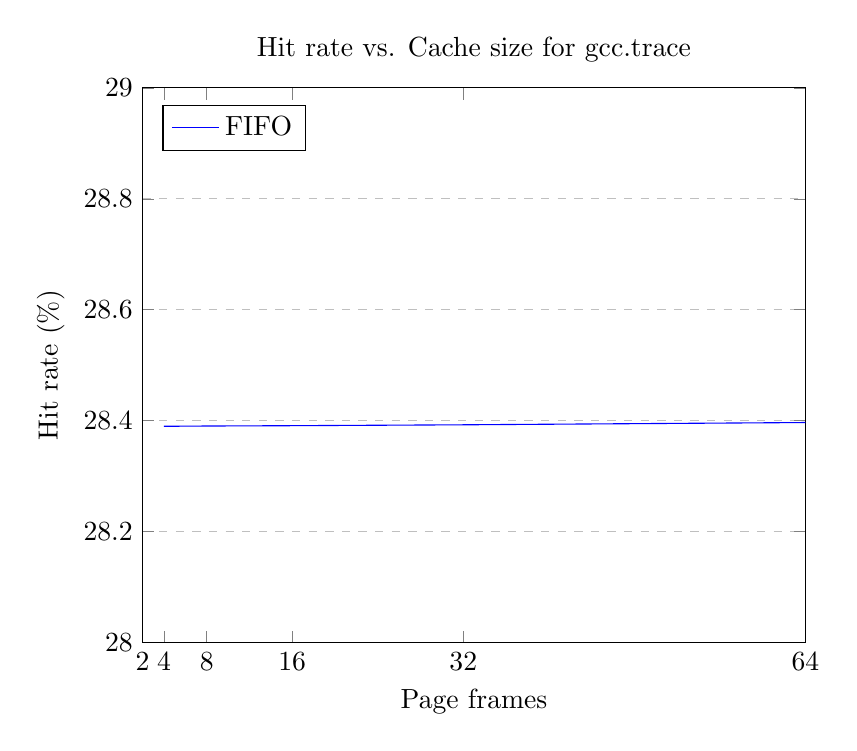
\begin{tikzpicture}
	\begin{axis}[
		title={Hit rate vs. Cache size for gcc.trace},
		xlabel={Page frames},
		ylabel={Hit rate (\%)},
		xmin=2, xmax=64,
		ymin=28, ymax=29,
		xtick={2, 4, 8, 16, 32, 64},
		legend pos=north west,
		ymajorgrids=true,
		grid style=dashed,
	]
	
	\addplot[
		color=blue,
	]
	coordinates {
		(4, 28.3898) (8, 28.3903) (16, 28.3909) (32, 28.3925) (64, 28.3966) (128, 28.4032) (256, 28.4212)
	};
	\legend{FIFO}
	
	\end{axis}
	\end{tikzpicture}
	
	
	\end{center}


	\section{Conclusion}
	The statistics we gathered from our simulations mainly matched what was hypothesized, that paging does help up to a point, and then after that point the optimization sort of plateaus. However smaller page frame sizes definitely show a negative impact on the system across any type of approach. VMS performed the best as it is the one with the most complexity in terms of allowing processes to reclaim memory that was about to be written to disk, helping prevent a ``miss'' to the hard disk. LRU came in second which is to be expected as it takes advantage of the previously mentioned spatial locality. While FIFO came in last (but not by as much as we expected on the bigger sizes) because it is the most simplest ``quick and dirty'' (pun not intended) page replacement algorithm aside from randomly evicting page entries.
	
\end{document}